\begin{enumerate}[label=\thesubsection.\arabic*.,ref=\thesubsection.\theenumi]
\numberwithin{equation}{enumi}

\item
Consider a unity feedback control system as shown in Fig.  \ref{fig:ee18btech11038}. Find the value of K that results in a phase margin of the system to be 30\degree.

\begin{figure}[!ht]
	\begin{center}
		
		\resizebox{\columnwidth}{!}{%\begin{figure}
\tikzstyle{block} = [draw, fill=blue!20, rectangle, 
    minimum height=1cm, minimum width=1cm]
\tikzstyle{sum} = [draw, fill=blue!20, circle, node distance=1cm]
\tikzstyle{input} = [coordinate]
\tikzstyle{output} = [coordinate]
\tikzstyle{pinstyle} = [pin edge={to-,thin,black}]

% The block diagram code is probably more verbose than necessary
\begin{tikzpicture}[auto, node distance=2cm,>=latex']
    % We start by placing the blocks
    \node [input, name=input] {X(s)};
    \node [sum, right of=input] (sum) {};
    
    \node [block, right of=sum] (system) {${Ke^{-s}}/s$ };
   
    % We draw an edge between the controller and system block to 
    % calculate the coordinate u. We need it to place the measurement block. 
    
    \node [output, right of=system] (output) {};
    \node [block, below of=system] (measurements) {1};

    % Once the nodes are placed, connecting them is easy. 
    \draw [draw,->] (input) -- node {$U(s)$} (sum);
    \draw [->] (sum) -- node {} (system);
    \draw [->] (system) -- node [name=y] {$Y(s)$}(output);
    \draw [->] (y) |- (measurements);
    \draw [->] (measurements) -| node[pos=0.99] {$-$} 
        node [near end] {} (sum);
\end{tikzpicture}
%\end{figure}}
	\end{center}
\caption{}
\label{fig:ee18btech11038}
\end{figure}

\solution Given $H\brak{s} = 1$ and $G\brak{s}$ = ${Ke^{-s}}/s$

Phase Margin\brak{PM} is defined as-
\begin{align}
\label{eq:PM_eq}
 PM &=\phi -\brak{-180\degree}
\\
\implies \phi + 180\degree 
\end{align}

where, 
\begin{align}
\label{eq:crossover_eq}
\phi = \angle G\brak{j\omega_{gc}}H\brak{j\omega_{gc}}
\end{align}
$\omega_{gc}$ is the gain-cross over frequency.

\item Find $\omega_{gc}$.
\\
\solution
\begin{align}
\abs{G\brak{j\omega_{gc}}H\brak{j\omega_{gc}}} &= 1
\\
\implies \abs{\frac{{Ke^{-j\omega_{gc}}}}{j\omega_{gc}}} &= 1
\\
\implies \omega_{gc} = K  \quad Assuming\, K>0
\end{align}
\item Find $\phi$.
\\
\solution 
\begin{align}
\label{eq:PM_in_K}
\phi &= \angle G\brak{j\omega_{gc}}H\brak{j\omega_{gc}} \quad
\\
\implies \angle \frac{{Ke^{-jK}}}{jK} \quad\quad
\\
\implies -90\degree - K\brak{180/\pi}
\end{align}
\item By \eqref{eq:PM_eq}
\begin{align}
    PM &= 30\degree
    \\
    by \eqref{eq:PM_in_K} \quad K = \pi/3
\end{align}
\item Verify result by plotting the gain and phase plots of $G\brak{j\brak{\omega}}$ 
\\
\solution The following code plots Fig. \ref{fig:ee18btech11038_graph}

\begin{lstlisting}
codes/ee18btech11038_plot.py
\end{lstlisting}
The Phase plot is as shown-
\begin{figure}[!h]
  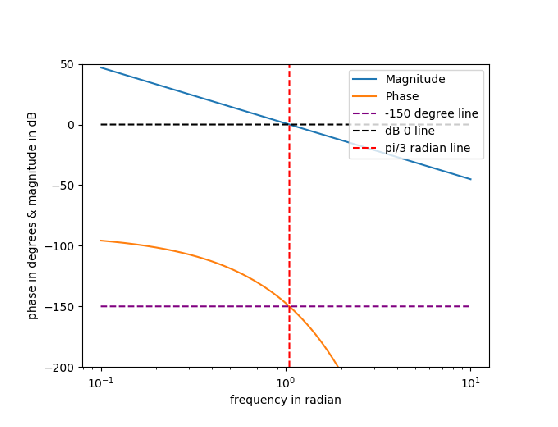
\includegraphics[width=\columnwidth]{./figs/ee18btech11038_graph.eps}
  \caption{}
  \label{fig:ee18btech11038_graph}
\end{figure}

\end{enumerate}
